\section{Results and conclusions}
In this section we present the comparisons of throughput and average buffer levels between continuous and in house developed discrete event simulation. In general two models are compared based on their results at steady state. Theoretically, a system is said to be at steady state, if all the state probabilities of the system approach a constant. For a small machine line with finite buffers the total state spaces can be equal to or more than gas molecules in a room. For present computational capabilities it will take forever to visit each of this state more than once, this condition cannot be fulfilled. However, when we run the simulations long enough certain line performance indicator such as throughput and average buffer levels approaches a constant value and this state is now mentioned as steady state.\par
\subsection{Results} 
We will start by comparing the results for a given simulation time $t_{simulation}$. The line parameters were generated by using the in house case generation method developed by Stan Gershwin. We simulated the same line for the constant simulated time $t_{simulation} = 10 days$, but we repeated the simulation for $10, 100, 1000$ times. The relative error in the throughput estimate in for all the three cases did not exceed $0.806\%$  indicating that $t_{simulation} = 10 days$ is long enough to achieve a constant throughput or a steady state in terms of throughput. In case of average buffer levels $(\bar{N})$ as presented in figure \ref{tab:constant_run_time} from the first row, we observe that continuous and discrete event simulation approach to same mean. However, their standard deviations are much higher, which indicated that buffer are not yet approaching to steady state. In the second row we show the buffer average occupancy calculated as $\bar{N} / N$. The buffer occupancy shows both the buffer varies from being empty to fulfill. The buffer distribution approach a normal distribution with increase in number of repetitions, this is due to rule of large numbers as we are simulating more number of random events during high repetitions. The mean of such normal distribution should indicate the steady state, but one cannot be sure until we reduce the variance of the distribution.  Hence, we decided to formulate a criterion to determine the run time for simulation such that average buffer levels approach a steady state. \par
\begin{table}[htbp]
    \centering
    \begin{tabular}{|p{5cm}|p{5cm}|p{5cm}|}
        \hline
        $t_{simulation} = 10 days$ & 
        $t_{simulation} = 100 days$ &
        $t_{simulation} = 1000 days$\\
        \hline  
        \parbox[c]{5cm}{\centering 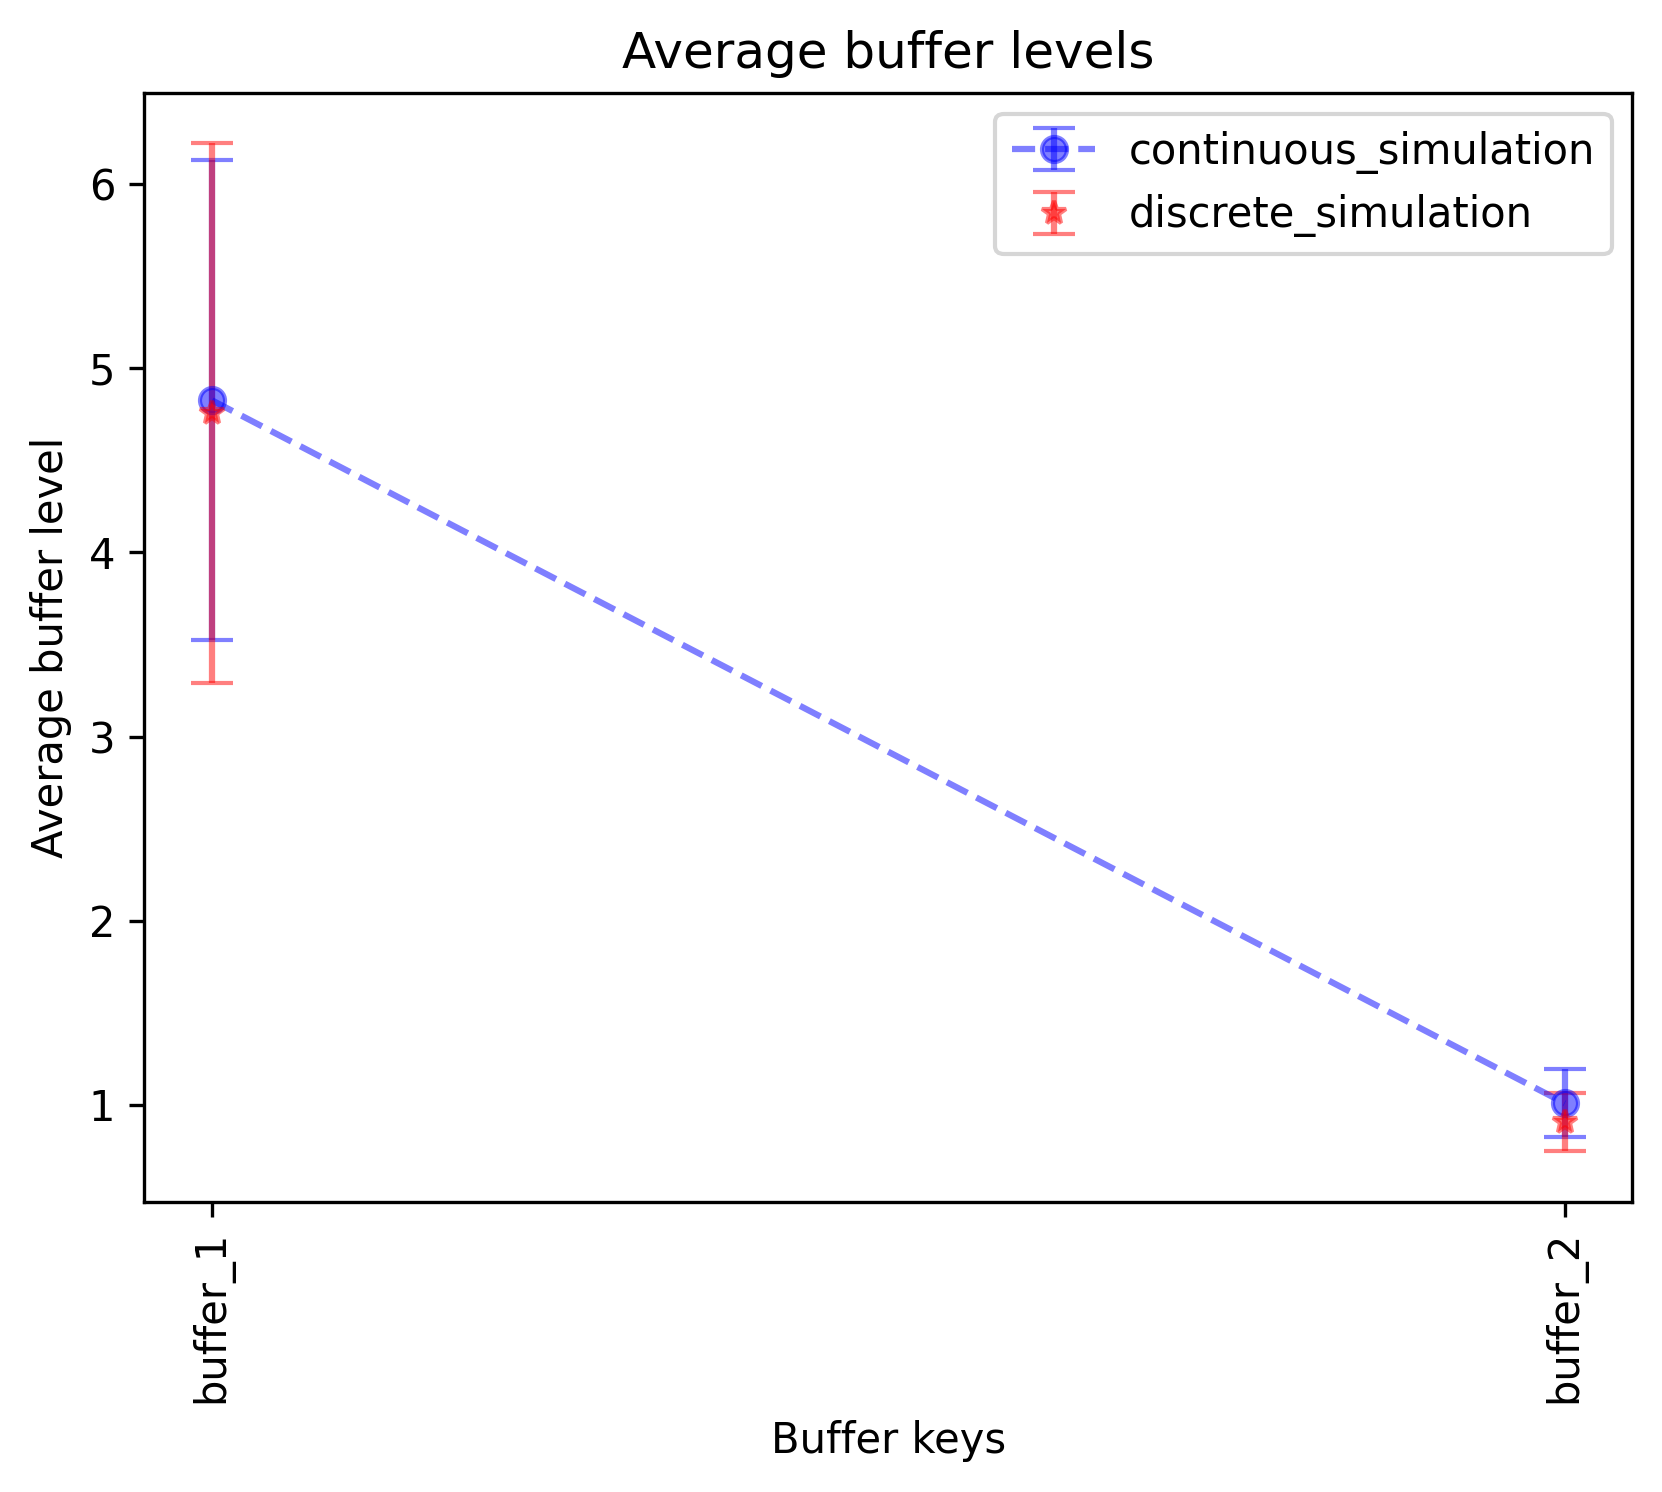
\includegraphics[width = 5cm]{figures/transfer_3_37_simple_10.png}} &
        \parbox[c]{5cm}{\centering 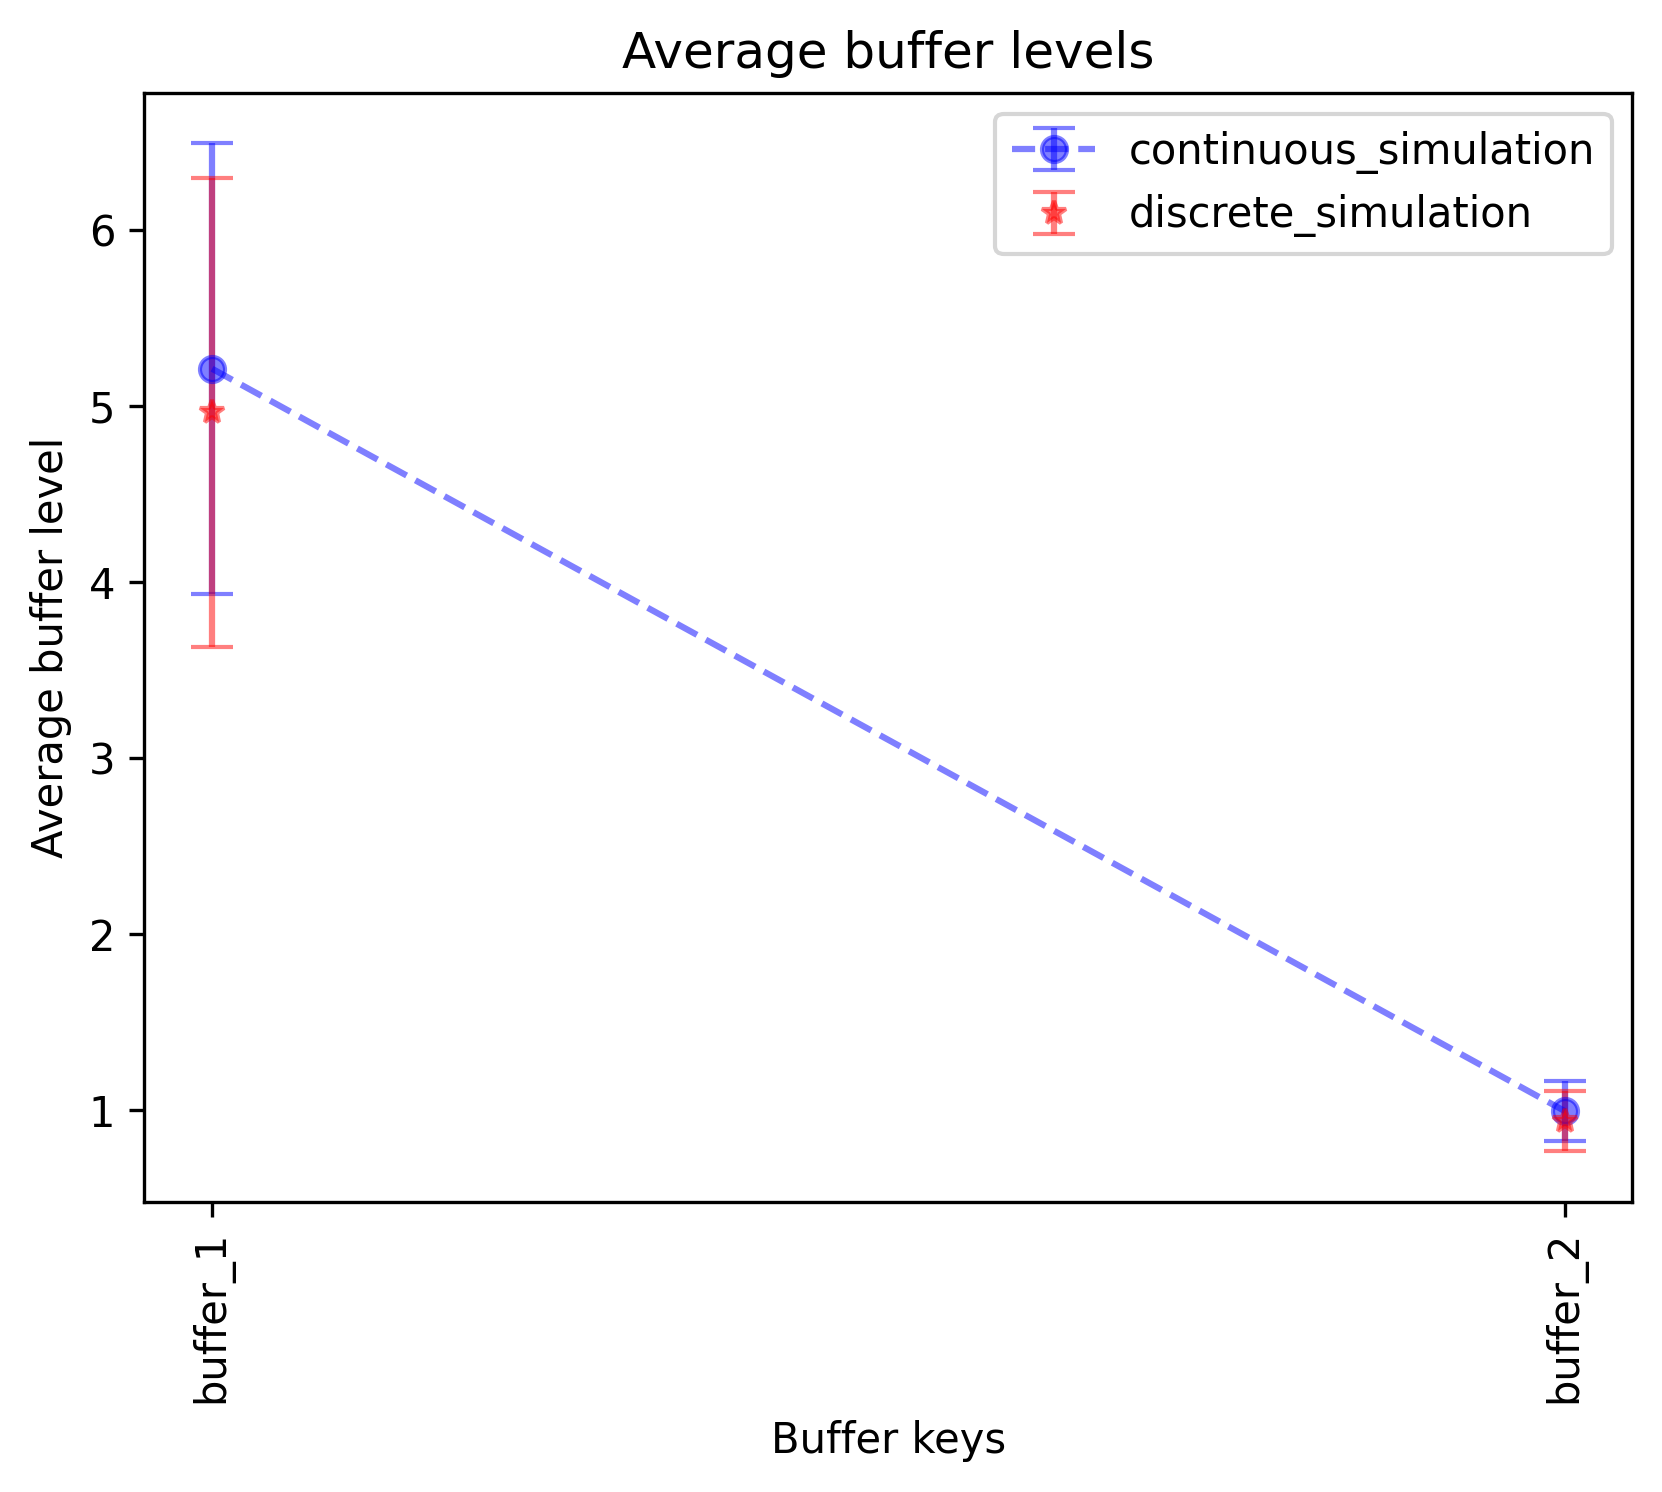
\includegraphics[width = 5cm]{figures/transfer_3_37_simple_100.png}} &
        \parbox[c]{5cm}{\centering 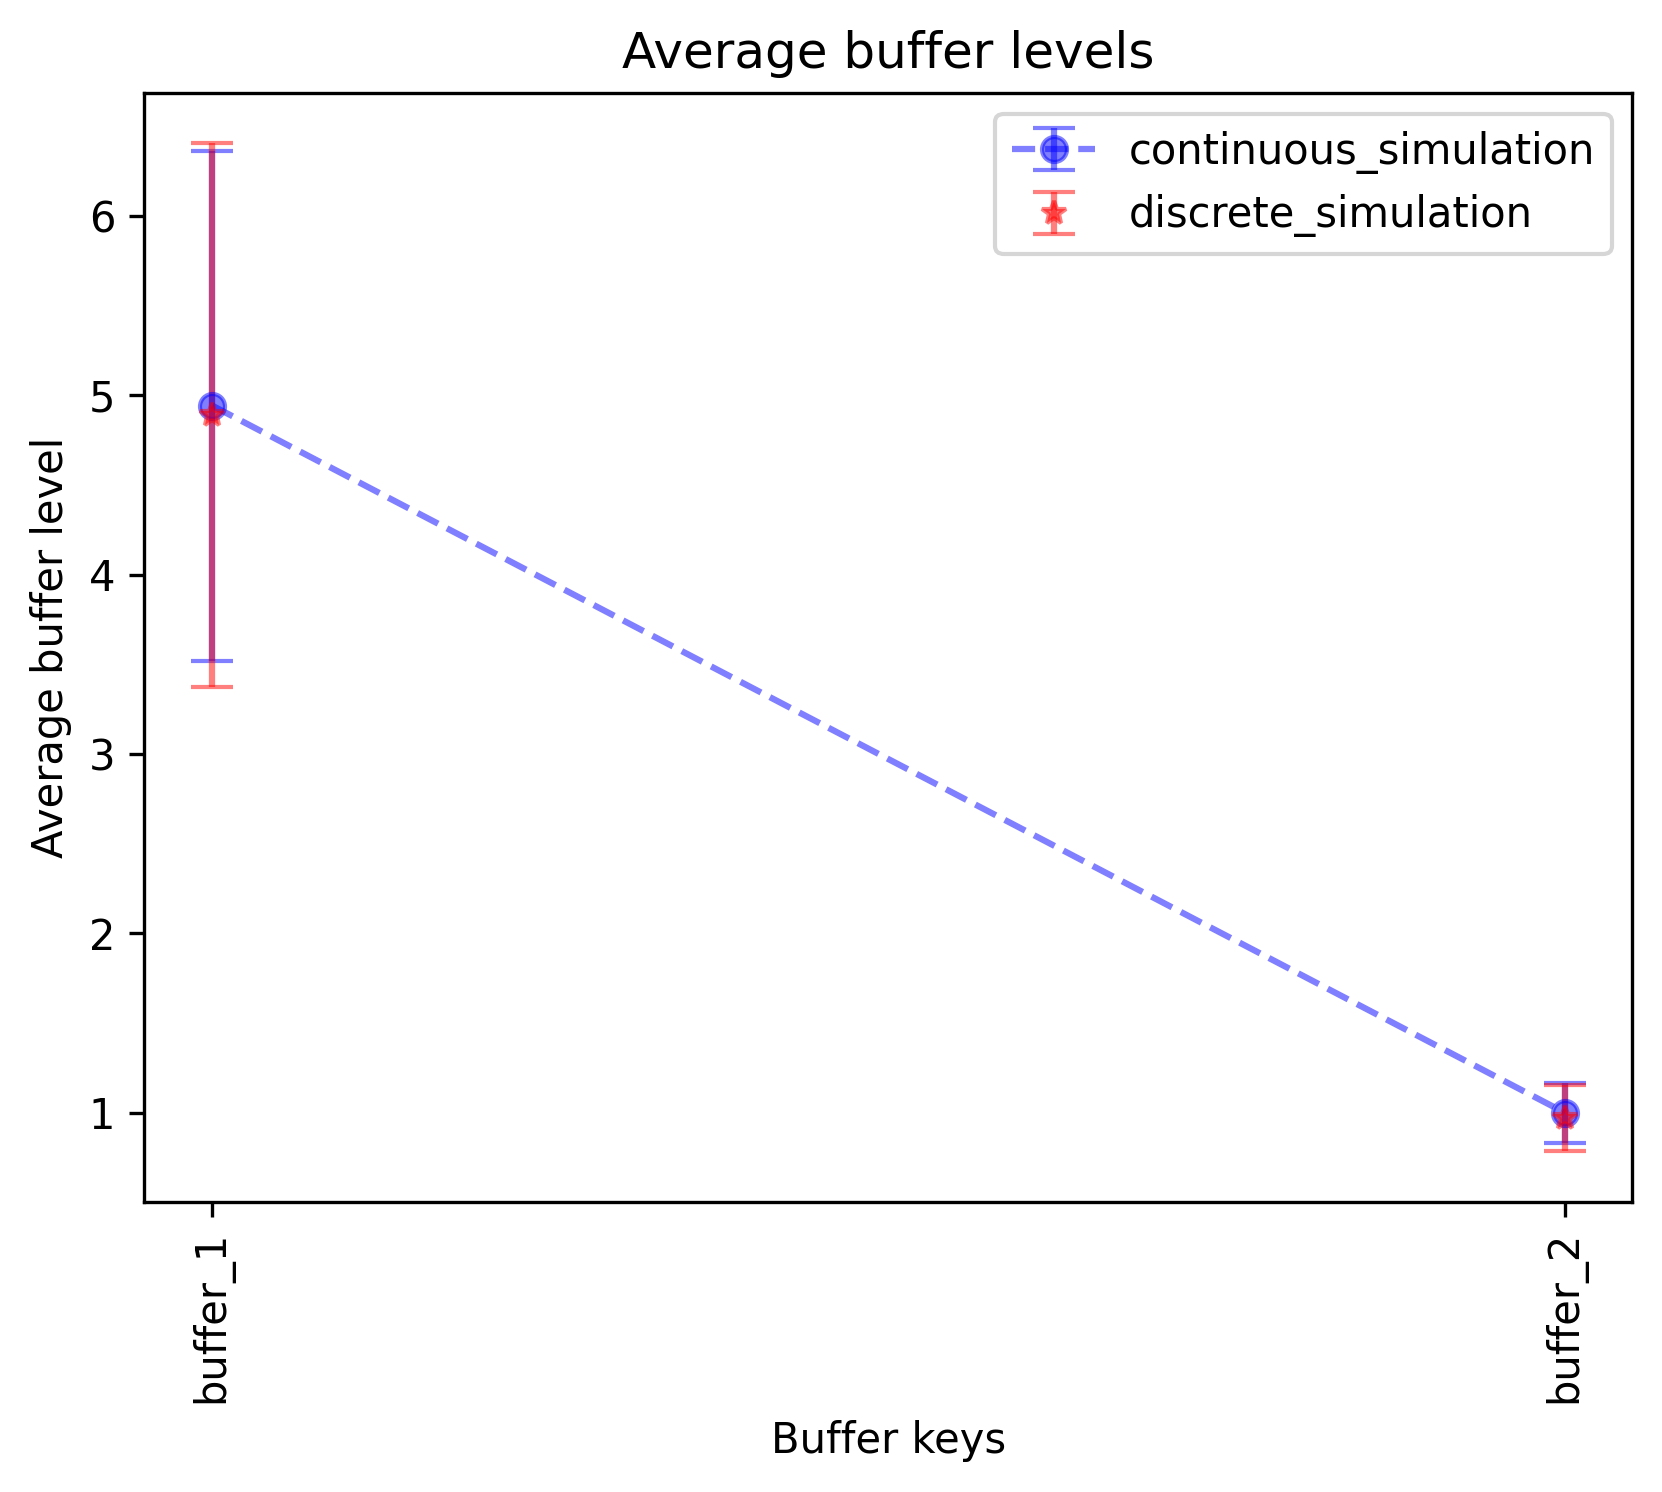
\includegraphics[width = 5cm]{figures/transfer_3_37_simple_1000.png}} \\
        \hline
        \parbox[c]{5cm}{\centering 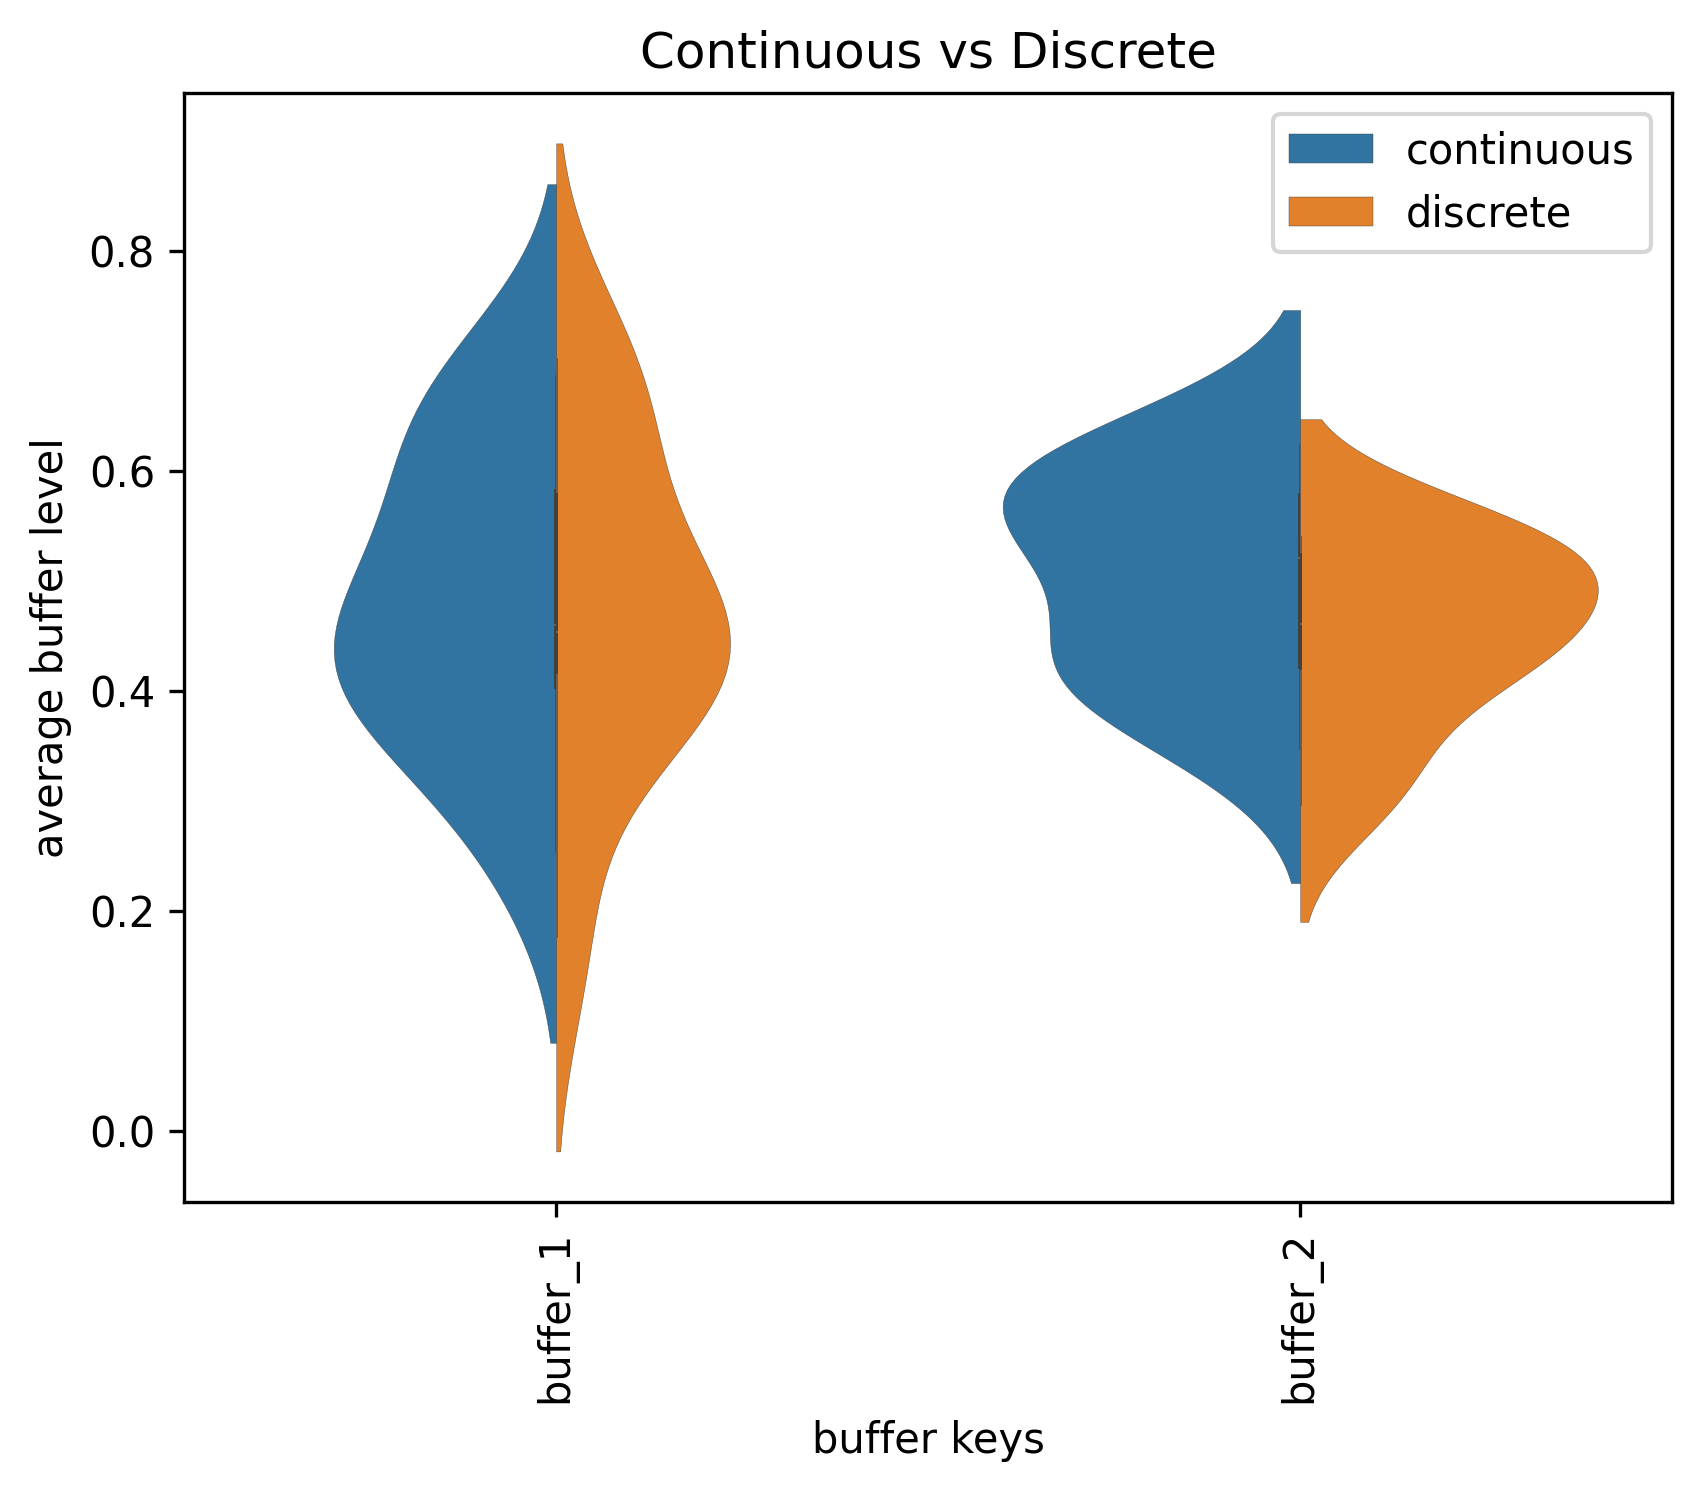
\includegraphics[width = 5cm]{figures/transfer_3_37_10.png}} &
        \parbox[c]{5cm}{\centering 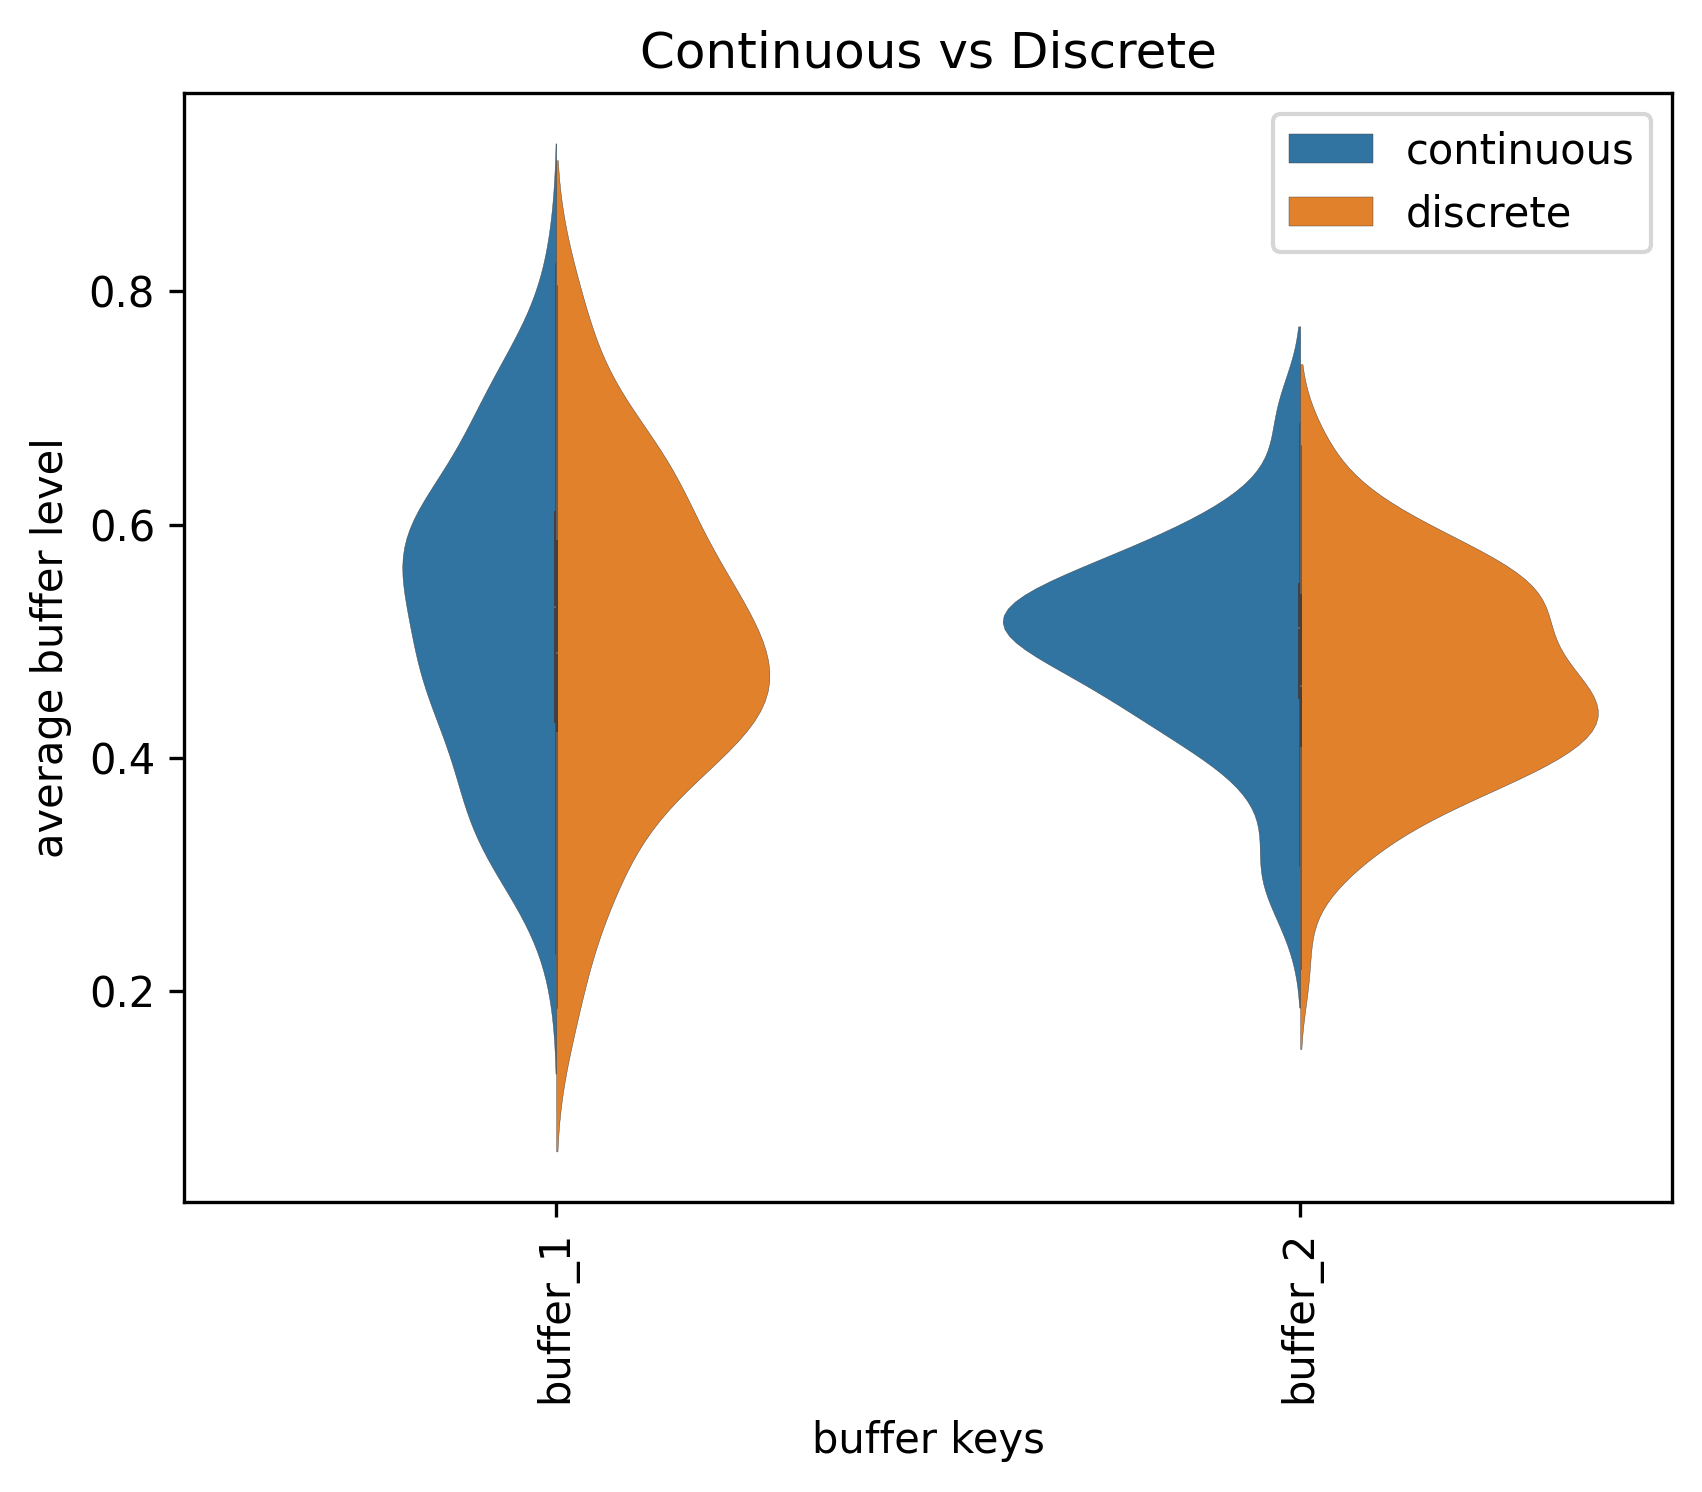
\includegraphics[width = 5cm]{figures/transfer_3_37_100.png}} &
        \parbox[c]{5cm}{\centering 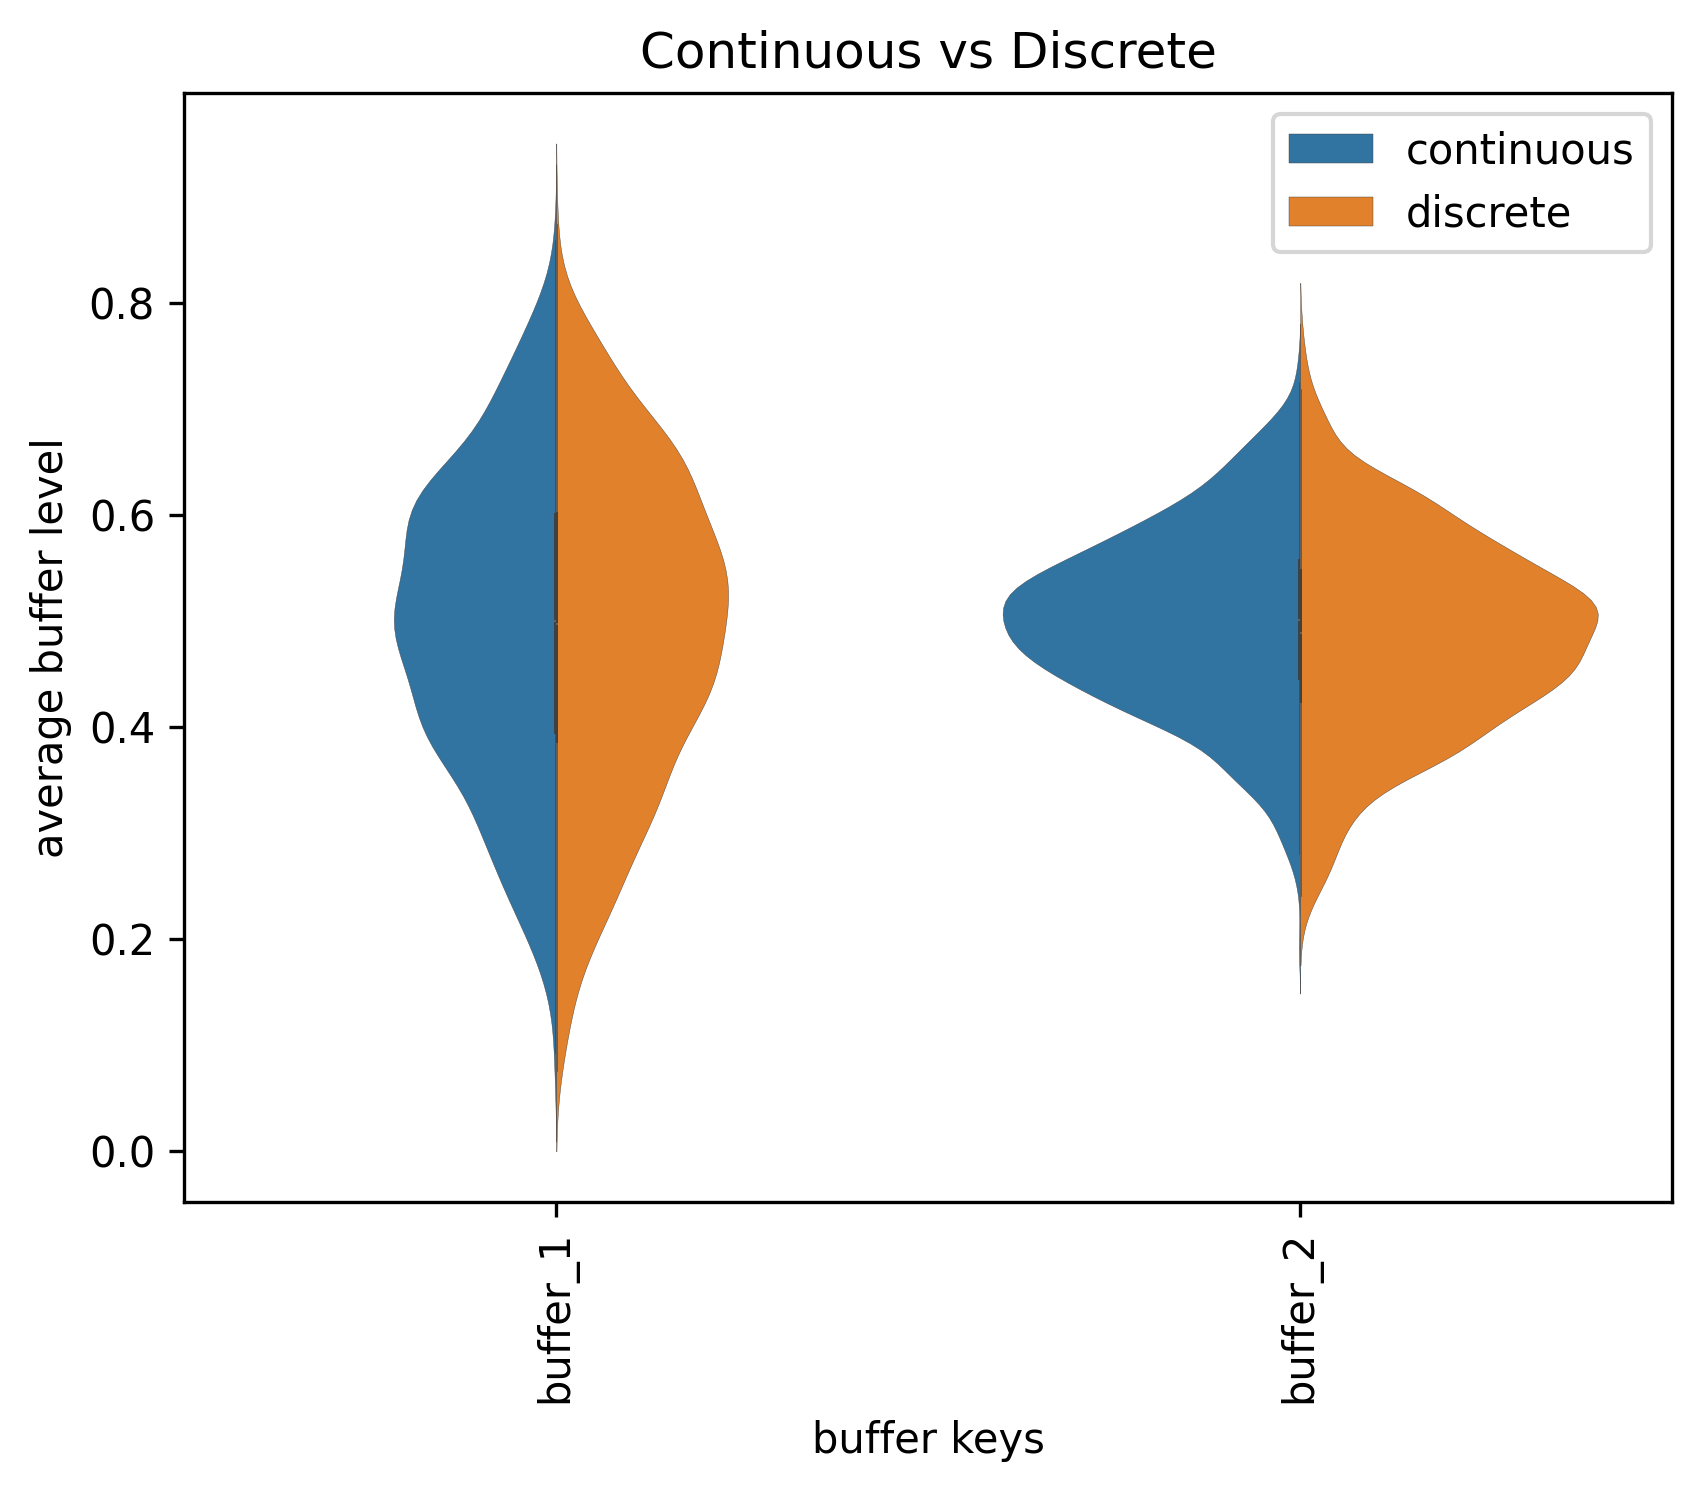
\includegraphics[width = 5cm]{figures/transfer_3_37_1000.png}} \\
        \hline
    \end{tabular}
    \caption{Distribution of average buffer levels with increase in number of repetition in simulation.}
    \label{tab:constant_run_time}
\end{table}
\textbf{Convergence criterion:}  Instead of terminating the simulation at a fixed run time, at end of simulation we re-run the simulation for three times to check the standard deviation of the throughput and average buffer levels over the three runs. If the standard deviation is less than $\epsilon = 10^{-5}$ we will terminate the simulation else we repeat the process by doubling the $t_{simulation} $. The results for a four and eight machine line are presented in figure \ref{tab:comparison}. The distributions have lower variation when compared to previous figure \ref{tab:constant_run_time}, providing more confidence on the steady state for the average buffer levels.
\begin{table}[htbp]
    \centering
    \begin{tabular}{|p{7cm}|p{7cm}|}
        \hline
        Four machine line & 
        Eight machine line \\
        \hline  
        \parbox[c]{7cm}{\centering 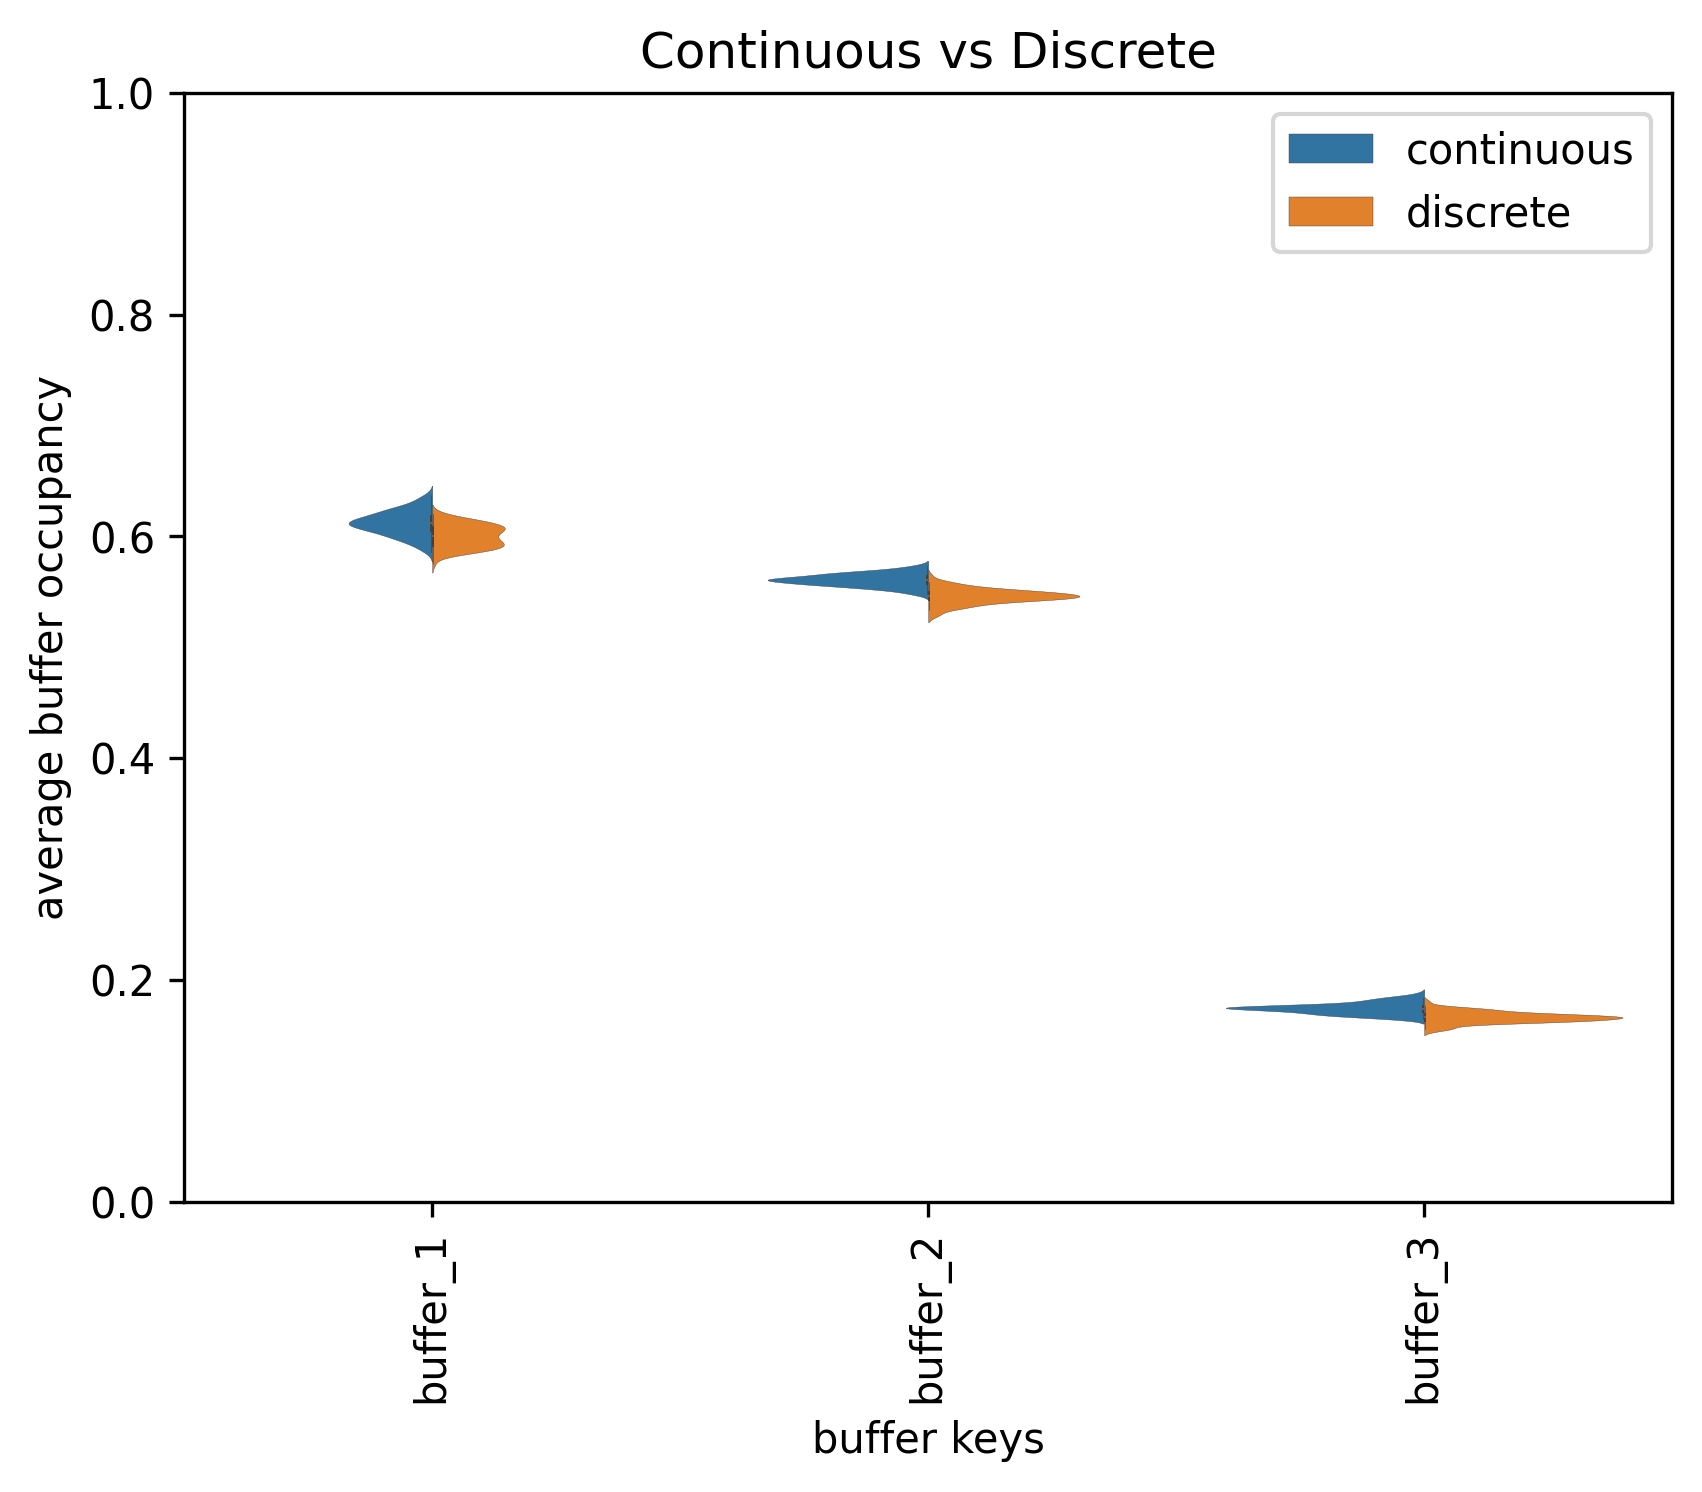
\includegraphics[width = 
        7cm]{figures/transfer_4_37_buffer_level_violin.png}} &
        \parbox[c]{7cm}{\centering 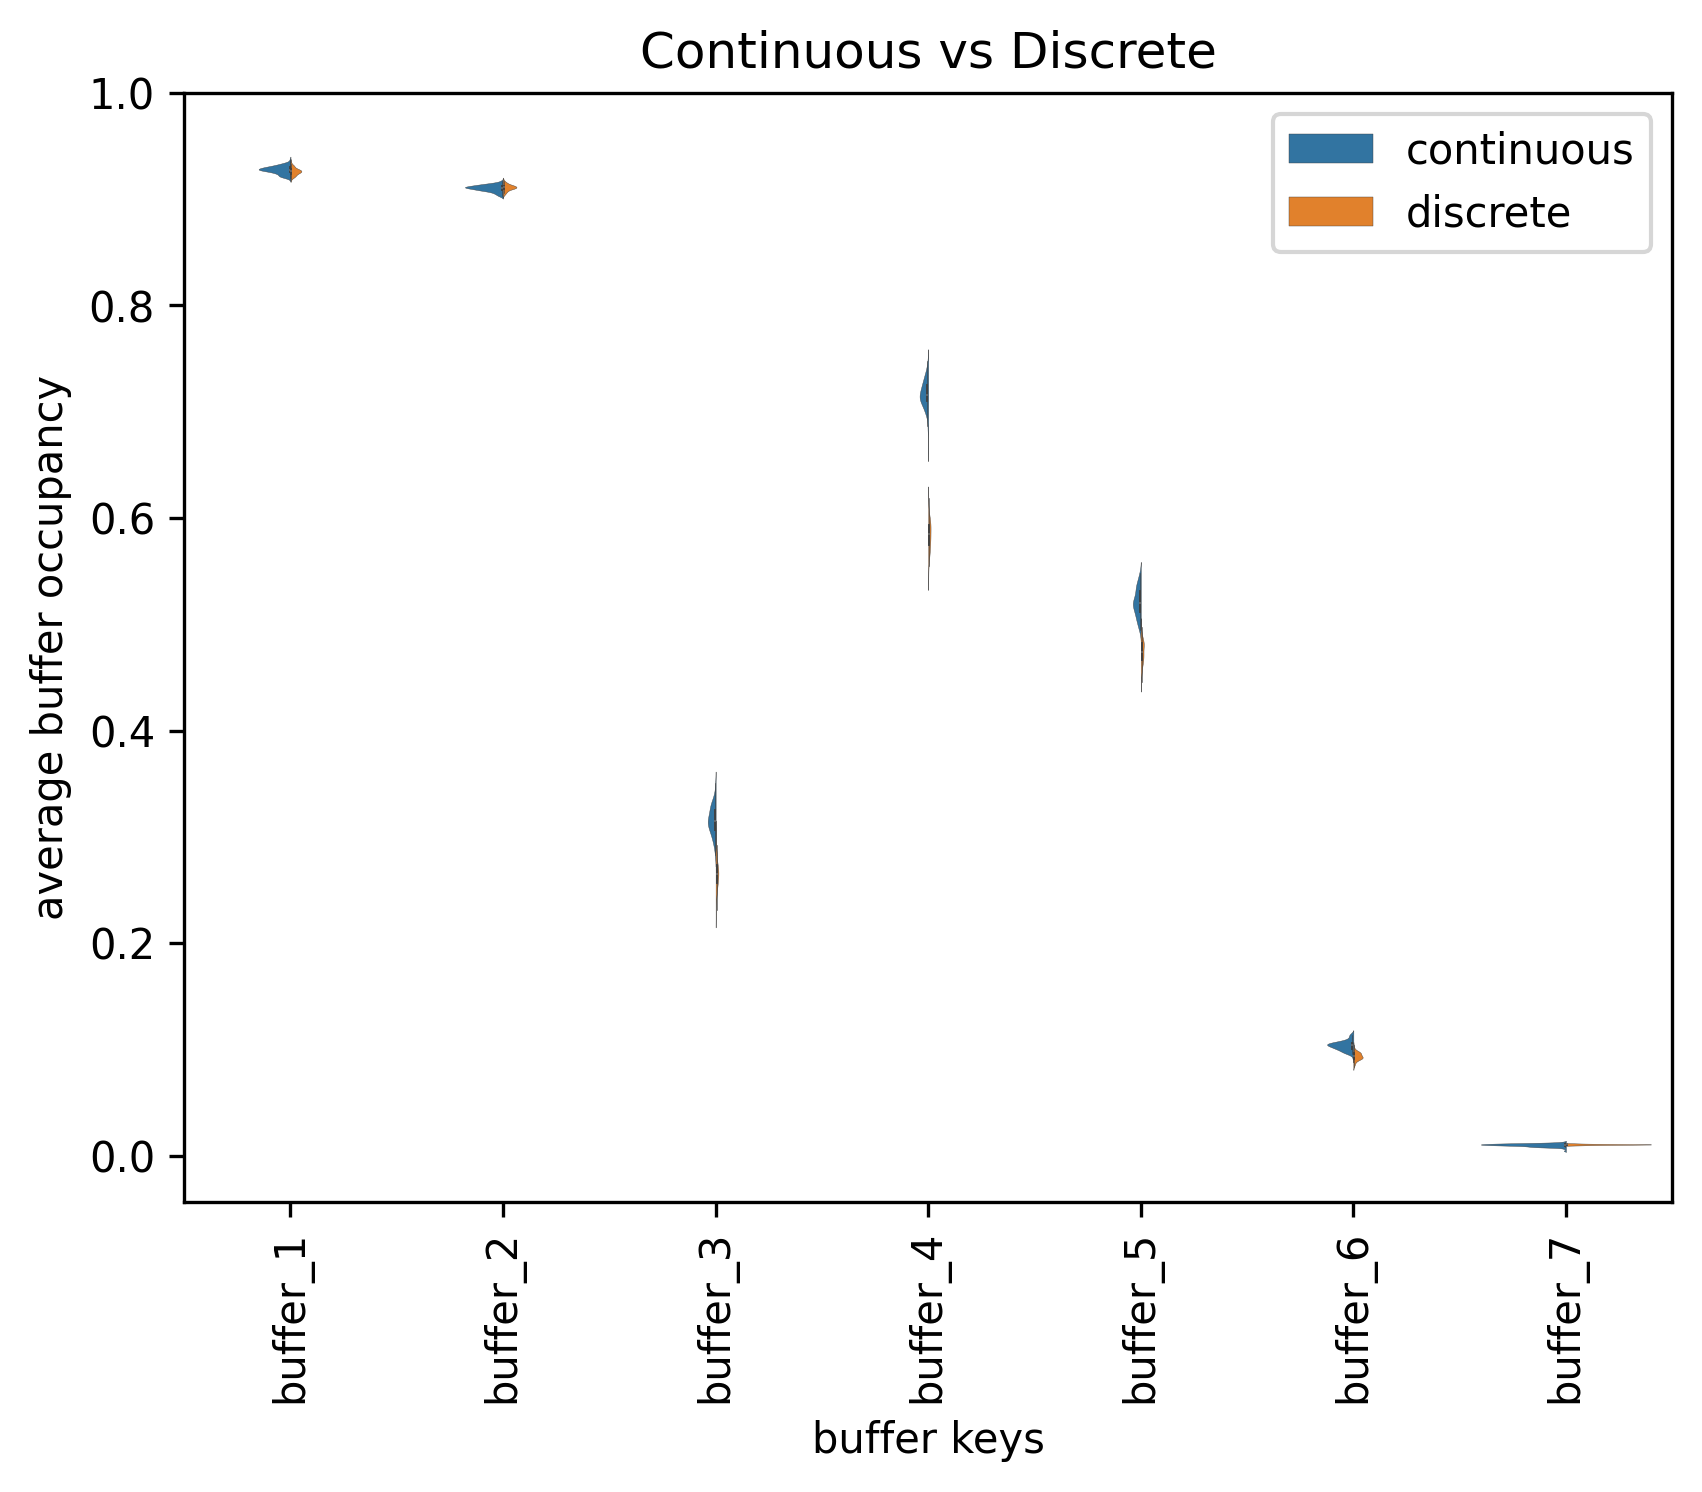
\includegraphics[width = 7cm]{figures/transfer_8_36_buffer_level_violin.png}} \\
        \hline
    \end{tabular}
    \caption{Distribution of average buffer levels for long lines.}
    \label{tab:comparison}
\end{table} 

\subsection{Conclusions}
In this study we presented an algorithm for continuous simulation model that can predict the average buffer levels and throughput. The predictions have minimum error when compared to discrete event simulation. Since, continuous and discrete simulations were written in different programming languages, the quantification of its computational efficiency is yet to be conducted. This work will be instrumental in developing later improvements to handle.\par
\begin{itemize}
    \item Multiple part type.
    \item Assembly, disassembly lines and loops.
\end{itemize} 
This work also provided a deep insight into mechanics of line and raised question on the evaluation of the steady state. 